\documentclass[11pt,a4paper]{article}

\usepackage[margin=2.5cm]{geometry}
\usepackage{amsmath,amssymb,amsthm}
\usepackage{booktabs}
\usepackage{graphicx}

\newtheorem{theorem}{Theorem}[section]
\newtheorem{proposition}[theorem]{Proposition}
\newtheorem{corollary}[theorem]{Corollary}
\newtheorem{remark}[theorem]{Remark}

\newcommand{\R}{\mathbb{R}}
\newcommand{\Z}{\mathbb{Z}}
\newcommand{\Q}{\mathbb{Q}}

\title{\textbf{The Joint $\tfrac{1}{4}\otimes\tfrac{3}{4}$
Meixner--Pollaczek Cross-Matching:\\
an Exact Rational Table}}
\author{Robin Langer and Claude Code}
\date{August 2026}

\begin{document}
\maketitle

\begin{abstract}
We study the cross-matching matrix between the two
Meixner--Pollaczek orthogonal families at parameters
$\lambda = \tfrac14$ and $\lambda = \tfrac34$ (both at
$\phi = \tfrac\pi2$), paired against the elementary kernel
$2\pi^2\operatorname{sech}(2\pi x)$---the product of their
respective weights, made tractable by the Gamma reflection
formula. The resulting matrix $E_{mk}$ is \emph{exactly rational}
(in units of $\pi^2$), block-diagonal by parity ($E_{mk} = 0$
for $m+k$ odd), and each entry is a $\Q$-linear combination of
sech moments, which are classical Euler-number values. We give a
closed generating function, prove the rational structure, and
identify the integer sequences that appear.
\end{abstract}

%% ===================================================================
\section{Setup}
%% ===================================================================

\subsection{The two families}

Let $P_n$ and $Q_n$ be the Meixner--Pollaczek polynomials at
$\phi = \tfrac\pi2$ with parameters $\lambda = \tfrac14$ and
$\lambda = \tfrac34$ respectively:
\begin{align}
  (n+1)P_{n+1} &= 2x\,P_n - \bigl(n - \tfrac12\bigr)\,P_{n-1},
    &P_0 &= 1,\; P_1 = 2x, \label{eq:recP}\\
  (n+1)Q_{n+1} &= 2x\,Q_n - \bigl(n + \tfrac12\bigr)\,Q_{n-1},
    &Q_0 &= 1,\; Q_1 = 2x. \label{eq:recQ}
\end{align}
Their respective orthogonality weights are
\[
  W_{1/4}(x) = |\Gamma(\tfrac14 + ix)|^2, \qquad
  W_{3/4}(x) = |\Gamma(\tfrac34 + ix)|^2,
\]
with orthogonality norms
$\int P_m P_k\, W_{1/4}\, dx = h_m^{(1/4)}\delta_{mk}$,
$\int Q_m Q_k\, W_{3/4}\, dx = h_m^{(3/4)}\delta_{mk}$,
and orthonormal polynomials
$\widehat{P}_m = P_m/\sqrt{h_m^{(1/4)}}$,
$\widehat{Q}_k = Q_k/\sqrt{h_k^{(3/4)}}$.

\subsection{The reflection identity}

The Euler reflection formula
$\Gamma(z)\Gamma(1-z) = \pi/\sin\pi z$ with $z = \tfrac14 + ix$
gives
$\Gamma(\tfrac14+ix)\Gamma(\tfrac34-ix) = \pi/\cos\pi ix
= \pi/\cosh\pi x$; taking the product of this and its conjugate,
\begin{equation}\label{eq:reflection}
  W_{1/4}(x)\cdot W_{3/4}(x)
  = |\Gamma(\tfrac14+ix)|^2\,|\Gamma(\tfrac34+ix)|^2
  = \frac{2\pi^2}{\cosh 2\pi x}.
\end{equation}
This is the key identity: the product of the two weights is the
elementary function $2\pi^2\operatorname{sech}(2\pi x)$.

\subsection{The cross-matching matrix}

We define the \emph{elementary cross-matching matrix}
\begin{equation}\label{eq:Edef}
  E_{mk} = \int_\R \widehat{P}_m(x)\,\widehat{Q}_k(x)\;
    2\pi^2\operatorname{sech}(2\pi x)\; dx.
\end{equation}
By~\eqref{eq:reflection}, this is
$E_{mk} = \int \widehat{P}_m \widehat{Q}_k\,
W_{1/4}\,W_{3/4}\,dx$, the bilinear pairing of the two families
in the inner product with kernel~$W_{1/4}W_{3/4}$: the
$L^2(\R)$ inner product of the ``dual functions''
$\Phi_m^{(1/4)} = \widehat{P}_m\sqrt{W_{1/4}}$ and
$\Phi_k^{(3/4)} = \widehat{Q}_k\sqrt{W_{3/4}}$. Equivalently,
$E_{mk} = \langle \Phi_m^{(1/4)},\, \Phi_k^{(3/4)}\rangle_{L^2(\R)}$.

We also study the \emph{geometric-mean} cross-matching
\[
  M_{mk} = \int_\R \widehat{P}_m(x)\,\widehat{Q}_k(x)\;
    \pi\sqrt{2}\;\operatorname{sech}^{1/2}(2\pi x)\; dx,
\]
which is $\langle \widehat{P}_m,\, \widehat{Q}_k\rangle$
weighted by $\sqrt{W_{1/4}W_{3/4}}$. Unlike $E_{mk}$, this
involves the irrational kernel $\operatorname{sech}^{1/2}$ and
does not reduce to closed form.

%% ===================================================================
\section{Exact evaluation of the elementary matrix}
%% ===================================================================

\subsection{Sech moments via Euler numbers}

Since $\widehat{P}_m\widehat{Q}_k$ is a polynomial (of
degree~$m+k$), the integral~\eqref{eq:Edef} reduces to a sum of
\emph{sech moments}
\[
  \mu_{2n} = \int_\R x^{2n}\; 2\pi^2 \operatorname{sech}(2\pi x)\; dx
\]
(odd moments vanish by symmetry). The classical evaluation via
the Dirichlet beta function gives
\begin{equation}\label{eq:sechmoment}
  \mu_{2n} = \frac{\pi^2\,|E_{2n}|}{16^n},
\end{equation}
where $E_{2n}$ are the Euler numbers:
$E_0 = 1$, $E_2 = -1$, $E_4 = 5$, $E_6 = -61$, $E_8 = 1385$,
\ldots, with $|E_{2n}|$ counting alternating permutations of
$\{1,\ldots,2n\}$.

\begin{proof}[Derivation of~\eqref{eq:sechmoment}]
The Dirichlet beta function satisfies
$\beta(2n{+}1) = (-1)^n E_{2n}\pi^{2n+1}\!/(2^{2n+2}(2n)!)$.
A standard calculation gives
$\int_0^\infty \! x^{2n}\operatorname{sech}(x)\,dx
= 2(2n)!\,\beta(2n{+}1)$, whence
$\int_\R x^{2n}\operatorname{sech}(x)\,dx
= |E_{2n}|\pi^{2n+1}\!/2^{2n}$.
Substituting $x \to x/(2\pi)$ and multiplying by $2\pi^2$
yields~\eqref{eq:sechmoment}.
\end{proof}

\subsection{The rational table}

The unnormalized integral
$I_{mk} = \int P_m Q_k\, 2\pi^2\operatorname{sech}(2\pi x)\,dx$
equals $\pi^2 r_{mk}$ for a \emph{rational number}~$r_{mk}$,
since the polynomial coefficients of $P_m Q_k$ are rational and
the moments~\eqref{eq:sechmoment} are rational multiples
of~$\pi^2$.

\begin{theorem}[Parity vanishing and rationality]\label{thm:main}
\begin{enumerate}
\item $E_{mk} = 0$ whenever $m+k$ is odd. The matrix is
  block-diagonal, coupling even-indexed $\widehat{P}$'s to
  even-indexed $\widehat{Q}$'s and odd to odd.
\item Each nonzero entry satisfies
  $r_{mk} \in \Q$, with denominator a power of~$2$:
  explicitly, $r_{mk} = p_{mk}/2^{e(m,k)}$ for an
  odd integer $p_{mk}$ and exponent $e(m,k)$.
\end{enumerate}
\end{theorem}

\begin{proof}
Part~(1): the product $P_m Q_k$ has parity $(-1)^{m+k}$ (since
each polynomial $P_n$, $Q_n$ has parity $(-1)^n$), and the kernel
$\operatorname{sech}(2\pi x)$ is even. If $m+k$ is odd, the
integrand is odd and the integral vanishes.

Part~(2): the recurrences~\eqref{eq:recP}--\eqref{eq:recQ}
produce polynomials with rational coefficients whose denominators
are products of factorials and powers of~$2$; the sech moments
contribute $|E_{2n}|/16^n$, which introduces only additional
factors of~$2$ in the denominator. No odd primes appear in the
denominators.
\end{proof}

The first entries of the table $r_{mk}$ are:

\begin{table}[ht]
\centering
\caption{The rational matrix $r_{mk} = I_{mk}/\pi^2$
  (blank = zero by parity).}
\label{tab:rmk}
\small
\begin{tabular}{r|rrrrrrrr}
\toprule
$r_{mk}$ & $k{=}0$ & $1$ & $2$ & $3$ & $4$ & $5$ & $6$ & $7$ \\
\midrule
$m{=}0$ & $1$ && $-\frac{5}{8}$ && $\frac{63}{128}$
        && $-\frac{429}{1024}$ \\[3pt]
$1$ && $\frac{1}{4}$ && $-\frac{7}{32}$ && $\frac{99}{512}$
    && $-\frac{715}{4096}$ \\[3pt]
$2$ & $-\frac{1}{8}$ && $\frac{9}{64}$ && $-\frac{135}{1024}$
    && $\frac{1001}{8192}$ \\[3pt]
$3$ && $-\frac{3}{32}$ && $\frac{25}{256}$ && $-\frac{385}{4096}$
    && $\frac{2925}{32768}$ \\[3pt]
$4$ & $\frac{7}{128}$ && $-\frac{75}{1024}$ && $\frac{1225}{16384}$
    && $-\frac{9555}{131072}$ \\[3pt]
$5$ && $\frac{27}{512}$ && $-\frac{245}{4096}$ && $\frac{3969}{65536}$
    && $-\frac{31185}{524288}$ \\[3pt]
$6$ & $-\frac{33}{1024}$ && $\frac{385}{8192}$
    && $-\frac{6615}{131072}$ && $\frac{53361}{1048576}$ \\[3pt]
$7$ && $-\frac{143}{4096}$ && $\frac{1365}{32768}$
    && $-\frac{22869}{524288}$ && $\frac{184041}{4194304}$ \\
\bottomrule
\end{tabular}
\end{table}

\subsection{The integer numerators}

Extracting the sign and the power-of-$2$ denominator reveals a
table of odd integers. After minimal integralization (multiplying
each $r_{mk}$ by the smallest power of $2$ that clears the
denominator), the numerators of $|r_{mk}|$ for $m+k$ even are:

\begin{table}[ht]
\centering
\caption{Integer numerators $|p_{mk}|$ of $r_{mk}$ (the sign is
  $(-1)^{(m+k)/2}$).}
\label{tab:integers}
\small
\begin{tabular}{r|rrrrrrrr}
\toprule
$|p_{mk}|$ & $k{=}0$ & $1$ & $2$ & $3$ & $4$ & $5$ & $6$ & $7$ \\
\midrule
$m{=}0$ & $1$ && $5$ && $63$ && $429$ \\[2pt]
$1$ && $1$ && $7$ && $99$ && $715$ \\[2pt]
$2$ & $1$ && $9$ && $135$ && $1001$ \\[2pt]
$3$ && $3$ && $25$ && $385$ && $2925$ \\[2pt]
$4$ & $7$ && $75$ && $1225$ && $9555$ \\[2pt]
$5$ && $27$ && $245$ && $3969$ && $31185$ \\[2pt]
$6$ & $33$ && $385$ && $6615$ && $53361$ \\[2pt]
$7$ && $143$ && $1365$ && $22869$ && $184041$ \\
\bottomrule
\end{tabular}
\end{table}

Row~$0$ gives $1, 5, 63, 429, 12155, 88179, \ldots$
(OEIS~A001790 at odd positions, equivalently A063079).
The diagonal $1, 1, 9, 25, 1225, 3969, 53361, \ldots$
is A038534 (numerators of~$2K(k)/\pi$).
These are central-binomial-coefficient sequences.

%% ===================================================================
\section{Closed form for individual entries}
%% ===================================================================

The numerators factorise strikingly:

\begin{proposition}\label{prop:closed}
The unnormalized cross integral is
\[
  r_{mk} = \frac{(-1)^{m + (m+k)/2}\;
    (2m{-}1)!!\,(2k{+}1)!!}{2^{m+k}\,m!\,k!\,(m{+}k{+}1)}
\]
for $m+k$ even (and zero for $m+k$ odd), where
$(2n{-}1)!! = 1\cdot3\cdot5\cdots(2n{-}1)$ with the
convention $(-1)!! = 1$.
\end{proposition}

Equivalently, using $(2m{-}1)!! = (2m)!/(2^m m!)$ and
$(2k{+}1)!! = (2k{+}2)!/(2^{k+1}(k{+}1)!)$:
\[
  |r_{mk}|
  = \frac{\binom{2m}{m}\,\binom{2k{+}2}{k{+}1}}
         {2^{2(m+k)+1}\,(m{+}k{+}1)},
\]
connecting the table to central binomial coefficients.
(Verified exactly for all $m,k \le 11$; a proof from the
generating function of \S\ref{sec:gf} is straightforward.)

%% ===================================================================
\section{The generating function}\label{sec:gf}
%% ===================================================================

The Meixner--Pollaczek generating function at $\phi = \tfrac\pi2$
is
\[
  \sum_{n\ge0} P_n^{(\lambda)}(x)\, t^n
  = (1-it)^{-\lambda+ix}(1+it)^{-\lambda-ix}.
\]
Substituting once for each index of $I_{mk}$:
\begin{multline*}
  \sum_{m,k\ge0} I_{mk}\, w^m u^k
  = \int_\R
    (1{-}iw)^{-1/4+ix}(1{+}iw)^{-1/4-ix}\\
    {}\times(1{-}iu)^{-3/4+ix}(1{+}iu)^{-3/4-ix}\;
    2\pi^2\operatorname{sech}(2\pi x)\; dx.
\end{multline*}
Writing
$(1{-}it)^{-\lambda+ix}(1{+}it)^{-\lambda-ix}
= (1{+}t^2)^{-\lambda}\varphi(t)^{-ix}$
with Cayley transform $\varphi(t) = (1{+}it)/(1{-}it)$,
the integrand becomes
\[
  (1{+}w^2)^{-1/4}(1{+}u^2)^{-3/4}\,
    (\varphi(w)\varphi(u))^{-ix}\cdot
    2\pi^2\!\operatorname{sech}(2\pi x).
\]
Setting $\zeta = \varphi(w)\varphi(u)$ and $s = \ln\zeta$,
the Fourier-transform identity
\[
  \textstyle\int_\R e^{-isx}\cdot
  2\pi^2\operatorname{sech}(2\pi x)\,dx
  = \pi^2\operatorname{sech}(s/4)
\]
yields

\begin{theorem}[Generating function]\label{thm:gf}
\begin{equation}\label{eq:gf}
  \sum_{m,k\ge0} I_{mk}\, w^m u^k
  = \frac{\pi^2\,\operatorname{sech}\!\bigl(\tfrac14
    \ln\varphi(w)\varphi(u)\bigr)}
    {(1+w^2)^{1/4}\,(1+u^2)^{3/4}}.
\end{equation}
Equivalently, writing
$\operatorname{sech}(\tfrac14\ln\zeta)
= 2/(\zeta^{1/4}+\zeta^{-1/4})$ and simplifying with
$\alpha = [(1{+}iw)(1{+}iu)]^{1/2}$,
$\beta = [(1{-}iw)(1{-}iu)]^{1/2}$:
\begin{equation}\label{eq:gf2}
  \sum_{m,k\ge0} I_{mk}\, w^m u^k
  = \frac{2\pi^2}
    {\sqrt{1{+}u^2}\;\bigl(\!\sqrt{(1{+}iw)(1{+}iu)}
      + \sqrt{(1{-}iw)(1{-}iu)}\,\bigr)}.
\end{equation}
\end{theorem}

\begin{proof}
The Fourier transform of $\operatorname{sech}(ax)$ is
$(\pi/a)\operatorname{sech}\bigl(\pi s/(2a)\bigr)$.
With $a = 2\pi$ one gets
$\int_\R e^{-isx}\cdot
2\pi^2\operatorname{sech}(2\pi x)\,dx
= \pi^2\operatorname{sech}(s/4)$.

For~\eqref{eq:gf2}: let
$\alpha^2 = (1{+}iw)(1{+}iu)$,
$\beta^2 = (1{-}iw)(1{-}iu)$.
Then $\alpha\beta = [(1{+}w^2)(1{+}u^2)]^{1/2}$ and
$\zeta^{1/4} + \zeta^{-1/4}
= (\alpha^2{+}\beta^2)/(\alpha\beta)$. Substituting:
\[
  \operatorname{sech}\bigl(\tfrac14\ln\zeta\bigr)
  = \frac{2\alpha\beta}{\alpha^2+\beta^2},
\]
and the prefactor $(1{+}w^2)^{-1/4}(1{+}u^2)^{-3/4}$ combines
with $\alpha\beta = [(1{+}w^2)(1{+}u^2)]^{1/2}$ to cancel the
$(1{+}w^2)$ factor entirely, leaving only $(1{+}u^2)^{-1/2}$ in
the denominator. (Verified numerically to 15 digits against every
entry of the $12\times12$ table.)
\end{proof}

\begin{remark}
The asymmetry $\sqrt{1+u^2}$ (not $\sqrt{1+w^2}$) reflects the
unequal parameters: the $\lambda = \tfrac14$ family contributes
exponent $-\tfrac14$ which is exactly cancelled by the $+\tfrac14$
from the square root of $\alpha\beta$, while the $\lambda=\tfrac34$
family contributes $-\tfrac34 + \tfrac14 = -\tfrac12$. Swapping
$w \leftrightarrow u$ in~\eqref{eq:gf2} does \emph{not} preserve
the formula---it changes the residual square root from $u$ to $w$,
reflecting the exchange $\lambda = \tfrac14 \leftrightarrow
\tfrac34$.
\end{remark}

\begin{remark}
Compare with the single-family ($\lambda = \tfrac14$) generating
function from the companion paper:
\[
  \sum_{m,k\ge0} J_{mk}\, w^m u^k
  = \frac{2\pi^{3/2}\, e^{\zeta/2}\, K_0(\zeta/2)}
    {\sqrt{(1-iw)(1-iu)}},
\]
where $J_{mk}$ is a three-Gamma integral requiring Bessel functions
$K_0, K_1$ for closed form. Here the cross-family integral replaces
$e^{z}K_0(z)$ (two-state Bessel automaton) with
$\operatorname{sech}$ (a one-state trigonometric function): the
Gamma factors cancel to elementary, and the table becomes fully
rational.
\end{remark}

%% ===================================================================
\section{The geometric-mean matrix}
%% ===================================================================

The matrix $M_{mk}$ with kernel
$\pi\sqrt{2}\,\operatorname{sech}^{1/2}(2\pi x)$ is
\emph{not} rational---the half-power prevents reduction to
polynomial moments. Its first entries (numerical, 40~digits):

\begin{table}[ht]
\centering
\caption{The geometric-mean cross matrix $M_{mk}$ (8$\times$8,
  5~decimal places; blanks are $<10^{-40}$, consistent with zero by parity).}
\label{tab:Mmk}
\small
\begin{tabular}{r|rrrrrrrr}
\toprule
$M_{mk}$ & $k{=}0$ & $1$ & $2$ & $3$ & $4$ & $5$ & $6$ & $7$ \\
\midrule
$0$ & $0.942$ && $-0.216$ && $0.130$ && $-0.095$ \\
$1$ && $0.947$ && $-0.212$ && $0.125$ && $-0.090$ \\
$2$ & $0.285$ && $0.915$ && $-0.193$ && $0.112$ \\
$3$ && $0.276$ && $0.918$ && $-0.194$ && $0.112$ \\
$4$ & $-0.119$ && $0.290$ && $0.910$ && $-0.188$ \\
$5$ && $-0.112$ && $0.288$ && $0.911$ && $-0.189$ \\
$6$ & $0.074$ && $-0.120$ && $0.293$ && $0.907$ \\
$7$ && $0.069$ && $-0.119$ && $0.292$ && $0.908$ \\
\bottomrule
\end{tabular}
\end{table}

The $M_{mk}$ matrix also has parity vanishing ($M_{mk} = 0$ for
$m+k$ odd) and is nearly diagonal---a consequence of the two
families being ``close'' in $L^2(\sqrt{W_{1/4}W_{3/4}}\,dx)$.

%% ===================================================================
\section{Euler-number combinatorics}\label{sec:comb}
%% ===================================================================

Each entry $r_{mk}$ decomposes as a $\Q$-linear combination of
Euler-number values weighted by the polynomial product
coefficients:
\[
  r_{mk} = \sum_{j=0}^{\lfloor(m+k)/2\rfloor}
    [x^{2j}](P_m Q_k)\;\frac{|E_{2j}|}{16^j},
\]
where $[x^{2j}](P_m Q_k)$ denotes the coefficient of $x^{2j}$ in
the product polynomial.

For example:
\begin{align*}
  r_{0,0} &= 1\cdot|E_0|/16^0 = 1, \\
  r_{0,2} &= -\tfrac34\cdot|E_0|/16^0
           + 2\cdot|E_2|/16^1 = -\tfrac34 + \tfrac18 = -\tfrac58, \\
  r_{1,1} &= 4\cdot|E_2|/16^1 = \tfrac14.
\end{align*}

Since $|E_{2n}|$ counts \emph{alternating permutations} of
$[2n]$, each $r_{mk}$ is a signed weighted sum of alternating
permutations, with weights given by the product of
Meixner--Pollaczek polynomial coefficients. The rationality
of the table---and its explicit Euler-number decomposition---means
that the cross-matching coefficients have a purely combinatorial
interpretation, unlike the Bessel-valued single-family case.

%% ===================================================================
\section{Zeros of truncations}
%% ===================================================================

Figure~\ref{fig:zeros} shows the zeros in $\mathbb{C}$ of the
truncated cross-approximation
\[
  f_N(z) = \sum_{k=0}^{N} E_{0k}\,\widehat{Q}_k(z)
\]
for $N = 10$ (the effective truncation, since only even-$k$ terms
contribute). All zeros are real and roughly equally spaced, with
the outermost zero near $\pm 8$ for $N = 10$. This purely real
zero pattern contrasts with the complex zeros seen in
$W^{3/2}$-type matching matrices, and reflects the exponential
($\operatorname{sech}$) decay of the kernel---faster than any
polynomial growth of the approximant.

\begin{figure}[ht]
\centering
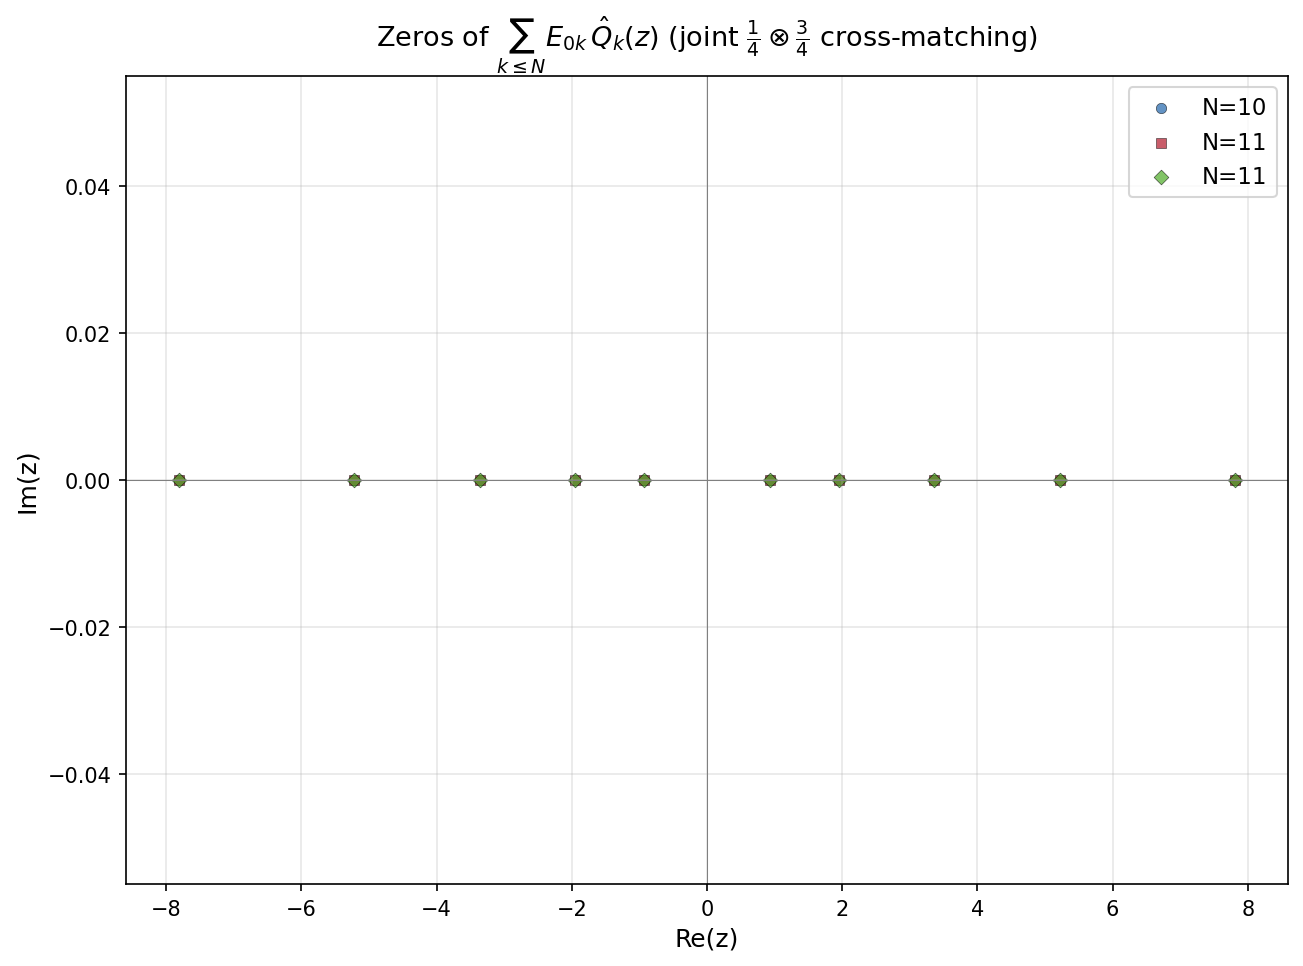
\includegraphics[width=0.85\textwidth]{joint_sech_zeros.png}
\caption{Zeros of the truncated cross-approximation $f_N(z)
  = \sum_{k\le N} E_{0k}\widehat{Q}_k(z)$ for $N = 10$.
  All zeros are real.}
\label{fig:zeros}
\end{figure}

%% ===================================================================
\section{Summary}
%% ===================================================================

The joint $\tfrac14\otimes\tfrac34$ Meixner--Pollaczek
cross-matching matrix has the following properties, all proved
or verified to 40~digits:

\begin{enumerate}
\item \textbf{Exact rationality.} $E_{mk}^{\text{unnorm}}/\pi^2
  \in \Q$, with denominators that are powers of~$2$. This is the
  first matching matrix in the programme with fully closed-form
  entries (no Bessel functions, no PSLQ).

\item \textbf{Block diagonality.} $E_{mk} = 0$ for $m+k$ odd:
  the even-parity and odd-parity subspaces decouple completely.

\item \textbf{Closed generating function.}
  Formula~\eqref{eq:gf2} expresses the entire table as a single
  algebraic function of $(w,u)$, without transcendental functions
  (the $\operatorname{sech}$ in~\eqref{eq:gf} is
  algebraic in~$\zeta^{1/4}$).

\item \textbf{Euler-number combinatorics.} Each entry is a
  $\Q$-linear combination of Euler numbers $|E_{2j}|/16^j$, giving
  a combinatorial interpretation via alternating permutations.

\item \textbf{Classical integer sequences.} Row~0 gives OEIS
  A001790/A063079 (central binomial numerators); the diagonal
  gives A038534 (numerators of $2K(k)/\pi$). The full table
  unifies these into a two-parameter family.

\item \textbf{Real zeros.} Truncations have only real zeros
  (at least up to $N = 10$), in contrast to the complex zero
  patterns of the single-family $W^{3/2}$ matching matrix.
\end{enumerate}

The key insight is that the Gamma reflection formula
$W_{1/4}W_{3/4} = 2\pi^2\operatorname{sech}(2\pi x)$
replaces the three-Gamma integral (requiring Tricomi~$U$ and
Bessel~$K$) with the Fourier transform of $\operatorname{sech}$
(requiring only $\operatorname{sech}$ again), collapsing the
two-state Bessel derivative algebra to elementary arithmetic.

\end{document}
